\documentclass[journal]{IEEEtran}
\hyphenation{op-tical net-works semi-conduc-tor}
\usepackage{amsmath}
\usepackage{amssymb}
\usepackage{graphicx}
\newcounter{OldYear}
\newcounter{NewYear}
\setcounter{OldYear}{2020}
\setcounter{NewYear}{2020}
\ifnum\month >9
	\stepcounter{NewYear}
\else
	\addtocounter{OldYear}{-1}
\fi

\newcommand{\seminar}{Seminar: Robotics and Artificial Intelligence \theOldYear /\theNewYear}


\begin{document}

\title{Uncertainty in Neural Networks: Review}

\author{Atharva Mahesh Kavitkar, Technische Universit\"{a}t Kaiserslautern}

\markboth{\seminar, RRLAB, Technische Universit\"{a}t Kaiserslautern}%
{Second Header}

\maketitle

\begin{abstract}
With the rapid adaptation of neural networks as the standard machine learning solution in various sectors of society, the question of their reliability in new and unknown environments has become increasingly relevant. Because of the tendency of neural networks to produce overconfident results in unfamiliar environments, mapping the confidence interval of a prediction from a neural network has become as important as the accuracy of its prediction itself. This paper reviews the two most prominent uncertainty quantification techniques in literature i.e. Bayesian approximation and Ensemble learning. The paper also investigates the real world application of these techniques comparing their relative performance on tasks related to robotics and computer vision (such as semantic segmentation, autonomous driving and image segmentation). In the end, the paper concludes by highlighting the challenges faced by uncertainty quantification methods and directions for future research in this field.
\end{abstract}

\begin{IEEEkeywords}
Neural networks, Uncertainty quantification, Bayesian modelling, Robotics, Computer vision.
\end{IEEEkeywords}

\IEEEpeerreviewmaketitle

\section{Introduction}

\IEEEPARstart{O}{ne} of the important requirements for machine learning models, is the explainability of the prediction process. Often the user of the prediction model is not only concerned with the accuracy of the prediction, but also with the explanation of the prediction for a new sample\cite{hariri2019uncertainty}. Models are susceptible to noise and biases inherited from the data and mathematical nature of the model causing unreliable predictions. It is therefore hugely valuable to evaluate uncertainty in a reliable manner prior to use of any AI-based system\cite{hariri2019uncertainty}.

One such area of application is robotics. Robots operate in an ambiguous environment. With view to organizing and decision-making, autonomous systems can only rely on noise perceptions and approximate models.
False decisions not only result in the failure to accomplish
the goal, but may also place human life at risk. Under these conditions, deep learning algorithms can only be completely implemented into robotic systems if a metric of predictive uncertainty is available.

Predictive variance in deep neural networks typically arises from two sources:data uncertainty and model uncertainty \cite{kabir2018neural}. The former is caused by noise in the results, normally because of the imperfections of the sensors. The latter is, instead, created by imbalances in the distribution or the incomplete nature of training data.
An uncommon sample, for instance, will have greater model uncertainty than a sample that occurs more frequently in the training results.
 Both types of ambiguity have an important role to play in Robot
 applications.
 It can never be believed that a sensor is Noise-free, and training datasets cannot be assumed to contain complete sample space.

As shown in Fig 1, Other scenarios that may
add to uncertainty include 
\begin{itemize}
    \item Noisy data: As a result of measurement inaccuracy, for example,
our observed labels can be noisy, contributing to aleatoric uncertainty. 
    \item Model parameter uncertainty: A large number of different models may be able to describe a
given dataset, in which case we could not be sure which model parameters to predict with. 
    \item Structural uncertainty: Which model system
are we going to use?
To extrapolate/interpolate well, how
do we decide our model \cite{kabir2018neural}? 
\end{itemize}

\begin{figure*}
    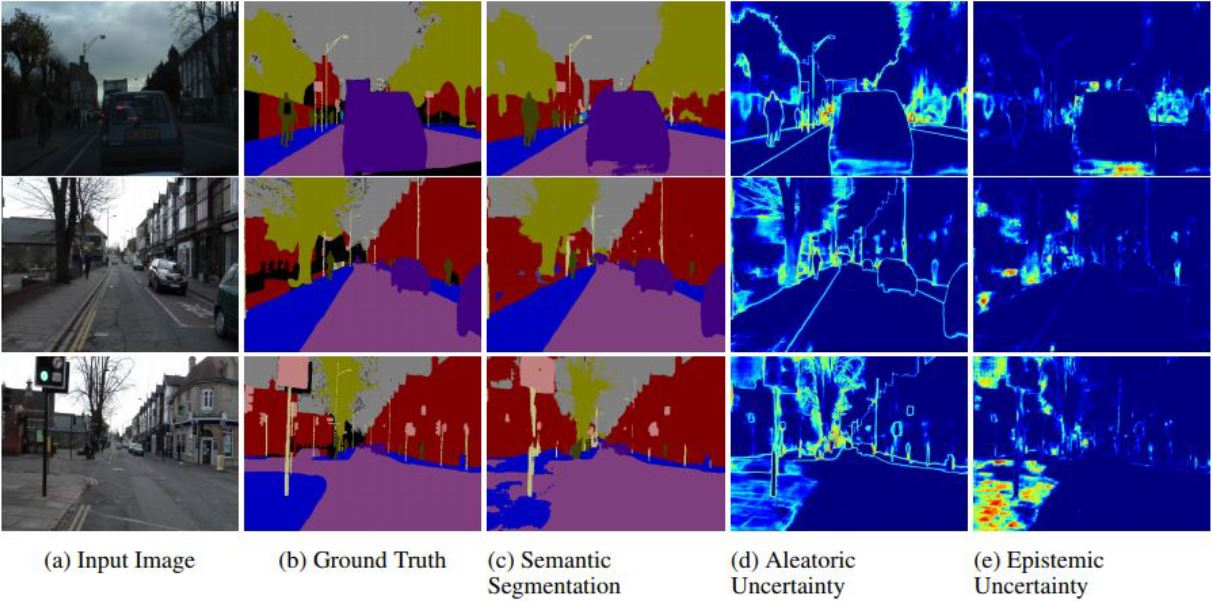
\includegraphics[scale=0.7]{figures/types_of_uncertainities.JPG}
    \caption{Types of uncertainties. \cite{kendall2019geometry}}
\end{figure*}

Remainder of the review is organised as follows. The Overview section provides the reader with the necessary concepts before exploring the techniques in further detail. A brief outline of the 2 major techniques discussed in this paper is also provided in the overview section. Next, each technique is discussed thoroughly in their respective sections. After studying the techniques, the next section discusses their application in robotics and computer vision. Conclusion and future work are outlined in the last section of the paper.

Main contributions of this review are:
\begin{itemize}
    \item Describe the different kinds of uncertainties pertaining to Neural Networks.
    \item Analyse the techniques used to quantify uncertainties.
    \item Discuss the application of these techniques in robotics and computer vision.
\end{itemize}
\section{Overview}
\subsection{Bayesian Modelling}
Given inputs $X = {x_1, . . . , x_N}$ and their corresponding outputs $Y = {y_1, . . . , y_N}$,
in Bayesian modelling we would like to find the parameters $\omega$ of a function $y = f_\omega(x)$ that are likely to have generated our outputs. Following the Bayesian approach we would put some prior distribution over the space of parameters, $p(\omega)$. This distribution is called the prior belief whose parameters are likely to have generated our data before we observe any data points. Once some data is observed, the prior belief will be transformed to fit the observed data points. For
this we further need to define a likelihood distribution $p(y|x,\omega)$, which we define as the probabilistic model by which the inputs generate the outputs given some parameter setting $\omega$.

\begin{equation*}
    p(y=d|x,\omega) = \frac{exp(f_{d}^{\omega}(x))}{\Sigma_{d'}exp(f_{d'}^{\omega}(x))}
\end{equation*}

Given a dataset X,Y, we then look for the posterior distribution over the space of
parameters by invoking Bayes’ theorem:

\begin{equation*}
    p(\omega|X,Y) = \frac{p(Y|X,\omega)p(\omega)}{p(Y|X)}
\end{equation*}

This distribution replicates the most probable function parameters given observed
data. The predicted output for a given input data point $x^*$ can be predicted by integrating:
\begin{equation*}
    p(y^*|x^*,X,Y) = \int p(y^*|x^*,\omega)p(\omega|X,Y)d\omega
\end{equation*}
This process is known as inference.

An important part of posterior evaluation is the model evidence:
\begin{equation*}
    p(Y|X) = \int p(Y|X,\omega)p(\omega)d\omega
\end{equation*}

Performing this integration is also called marginalising the likelihood over $\omega$.
For basic models, such as Bayesian
linear regression, marginalisation can be conducted analytically.
Marginalisation is the foundation of Bayesian
modelling, and we would want to marginalise over all uncertain parameters in an ideal world by averaging over all model parameter values $\omega$, each weighted by its probability
p($\omega$)\cite{abdar2020review}.

\subsection{Ensemble Techniques}
Although there has not been conducted a large scale research on uncertainty predictions in
general, the accuracy of predictive uncertainty estimation is a daunting activity.
Currently, two evaluation measures are applied for uncertain
ty estimation,
called calibration and domain shift \cite{pearce2018uncertainty}.
The functional implementations of Neural Networks(NNs)
are generally inspired by them.
The difference between highly probable predictions and arbitrary predictions is calculated by calibration.
The second principle involves the generalisation of domain
change predictive ambiguity, which estimates whether the network knows
what it really knows.
Predictive performance is improved
by an ensemble of models.
It is not clear, however, why and when an
ensemble of NNs will produce good estimates of uncertainty \cite{abdar2020review}. 
Bayesian Model Averaging (BMA) assumes that the actual model lies within the previous hypothesis class
and conducts soft model filtering to find the best single model within the class of hypotheses. On the other hand, ensembles
combine models to discover more accurate models. Therefore, ensembles
can be anticipated to be better when the true model
does not lie down within the hypothesis class.

\section{Bayesian Techniques}
\subsection{Bayesian Neural Networks}

Inspite of the effectiveness of traditional Deep Learning approaches in solving different real-word issues
, these methods do not provide details about the efficacy of their predictions\cite{jospin2020hands}.
Bayesian Neural Networks can be used to represent
the model parameters and mitigate this problem.
Bayesian Neural Networks are robust against overfitting and can
be trained on small and large datasets.

A Bayesian neural network is defined somewhat differently in the literature, but a standard concept (as represented in Fig 2) is that a stochastic artificial neural network trained with Bayesian inference is a Bayesian neural network.
Artificial neural networks (ANNs) have the
purpose of describing an arbitrary function $y=NN(x)$.
Using a succession of one input layer, a variety of hidden layers and
one output layer, typical ANNs (e.g. feedforward networks, repetitive networks, branched networks,...) are constructed.  Input variables are designated as $x$ and
output variables (predictions) are designated as $y$.
Each layer $l$ is defined in feedforward networks, the simplest architecture, as a linear
transformation of the previous one, followed by a nonlinear $nl$ operation (a.k.a activation function): 

\begin{equation*}
    l_0 = x
\end{equation*}
\begin{equation*}
    l_i = nl_i(W_il_{i-1} + b_i) \; \; \forall i \in [1,n]
\end{equation*}
\begin{equation*}
    y = l_n
\end{equation*}

The first step is the choosing of a deep neural
network architecture, i.e., a functional model, to construct a Bayesian Neural Networks(BNN).
Then a stochastic model needs to be selected, i.e. a prior distribution over the potential parametrization
of the model $p(\theta)$ and a prior confidence in the prediction accuracy of the $p(y|x,\theta)$ model\cite{jospin2020hands}.
It is possible to take the model parameterization to be the
hypothesis $H$ and the data $D$ as the training set.
We will define the model parameter as $\theta$ for the remainder of this section, and  $D$ has been used to
designate the training range, $D_x$ to designate the training features and $D_y$ has been used to designate the training marks.
This is to discriminate between the data
from the training and every input/output pair. Applying Bayes theorem, the Bayesian posterior can be formulated as:

\begin{equation*}
    p(\theta|D) = \frac{p(D_y|D_x,\theta)p(\theta)}{\int_\theta p(D_y|D_x,\theta')p(\theta')d\theta'} \propto p(D_y|D_x,\theta)p(\theta)
\end{equation*}

\begin{figure}[ht]
  \centering
  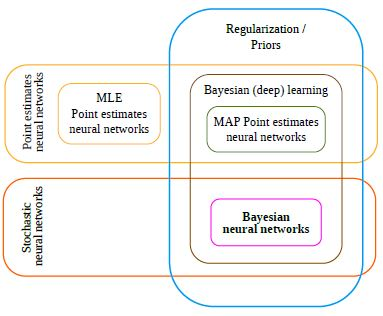
\includegraphics[width=85mm]{figures/BNN.JPG}
  \caption{Categorization of Bayesian Neural Networks\cite{jospin2020hands}}
\end{figure}

It is typically an intractable problem to compute this distribution, and also to sample it using
standard methods, especially because it is difficult to compute the evidence  $\int \theta p(D_y|D_x,\theta')p(\theta')d\theta'$.
Two methods are
capable of resolving this.
The first is to use a Markov Chain Monte Carlo algorithm, which requires the
posterior to be sampled explicitly, but a set of  samples $\theta$ must be cached.
The second is to use an approach called variational inference that
learns to estimate the exact posterior of a variational distribution $q \phi(\theta)$. 

\subsection{Monte Carlo dropout}

As mentioned earlier, the exact posterior inference is
difficult to compute, but it can be approximated.
Monte Carlo (MC) is an
efficient process in this respect.
MonteCarlo (MC) dropout has been implemented to combat this, and uses
dropout as a term of regularisation to measure the volatility of estimation.
Dropout is a reliable approach that has been
used extensively in DNNs to address over-fitting problems\cite{jospin2020hands}. 

\begin{figure}[ht]
  \centering
  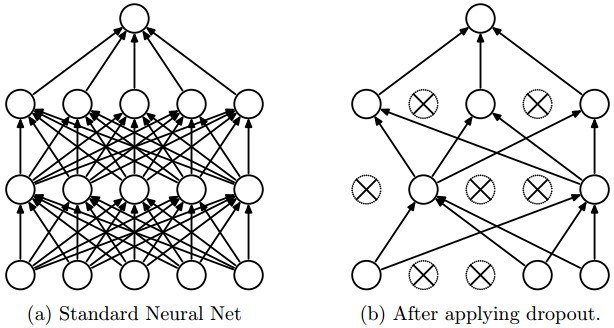
\includegraphics[scale=0.4]{figures/mc_dropout.JPG}
  \caption{Visual representation of Monte Carlo dropout}
\end{figure}

As shown in Fig 3, the dropout randomly loses any NN units during the training
period to keep them from co-tuning far too much.
Assume a NN with $L$ layers that denote the weight matrices, bias vectors and
dimensions of the $l^{th}$ layer with $W_l$, $b_l$ and $K_l$ respectively.
The NN output and the $i^{th}$ input $x_i(i = 1...N)$
reference class are represented by $\hat{y i}$ and $y_i$, respectively.
It is possible to write the
objective function using L2 regularisation as: 

\begin{equation*}
    L_{dropout} = \frac{1}{N}\sum_{i=1}^{N} E( y_i,\hat{y_i}) + \lambda \sum_{l=1}^{L} (||W_i||^2_2 + ||b_i||^2_2) 
\end{equation*}
Dropout samples binary variables for each input data and for each network unit on each layer (with the exception of the output layer),
with the likelihood of $p_i$ for the $i^{th}$ layer, if the value is 0, the unit $i$ for the input data is removed. For updating parameters, the same values
are used in the backward pass.

\subsection{Variational Inference}

Typically, the true posterior
$p(\omega|X,Y)$ cannot be analytically evaluated.
Instead, we define an approximate variational distribution $q \theta(\omega)$,
parameterized by $\theta$, whose structure is simple to test \cite{abdar2020review}.
We would like our approximate distribution to be as
similar as possible to the original model's posterior distribution.
Therefore, we minimise the divergence of Kullback-Leibler (KL) w.r.t.
$\theta$, intuitively a measure of correlation between two distributions: 
\begin{equation*}
    KL(q_\theta(\omega) || p(\omega|X,Y)) = \int q_\theta(\omega) log\frac{q_\theta(\omega)}{p(\omega|X,Y)}d\omega
\end{equation*}
Minimising the KL divergence allows us to approximate the predictive distribution as
\begin{equation*}
    p(y^*|x^*,X,Y) \approx \int p(y^*|x^*,\omega)q_\theta^*(\omega)d\omega = q_\theta^*(y^*|x^*)
\end{equation*}
The minimization of KL divergence is also analogous to optimising the
evidence lower bound (ELBO) w.r.t. the variational parameters defining $q \theta(\omega)$, 
\begin{equation*}
        L_{VI}(\theta) = \int q_\theta(\omega)logp(Y|X,\omega)d\omega - KL(q_\theta(\omega) || p(\omega)
\end{equation*}
\begin{equation*}
     L_{VI}(\theta) \leq logp(Y|X)
\end{equation*}
$logp(Y|X)$ is the log evidence
that determines the objective function.
In this last equation, maximising the first term (referred to as the expected log likelihood) encourages $q \theta(\omega)$ to describe the details well,
while minimising the second term (referred to as the previous KL) encourages $q_\theta(\omega)$ to be as similar to the prior as possible. 

This approach is referred to as variational
inference (VI), a common technique in Bayesian modelling\cite{posch2019variational}. The marginalisation is replaced by optimization by variational inference, i.e.
the estimation of integrals with that of derivatives is replaced.
But compared to the optimization methods often used in deep learning,
we optimise over distributions rather than point estimates in this environment.
This methodology retains many of Bayesian modeling's benefits (such as the balance between complex models and models
that describe the data well) and results in probabilistic models that capture the complexity of the model\cite{posch2019variational}. 

It is also much simpler to calculate
derivatives than integrals, which makes certain approximations tractable.
But even though for a wide class of models, this
method makes inference empirical, it still fails in certain aspects.
This method does not scale to massive data and does not adapt the technique
to dynamic models (models in which this last integral cannot be evaluated analytically)\cite{posch2019variational}. 

\subsection{Bayesian Convolutional Neural Networks}

At the end of the model alone, dropout is often
seen after inner-product layers in current convolutionary neural networks (CNNs) literature.
Before feeding it into a Bayesian NN, this can be seen as adding a finite deterministic transformation to the results. As such, parameter
instability for such models can still be obtained, but an important question is whether we should use approximate Bayesian inference over the complete CNN. \cite{kendall2019geometry}
Here, we want to integrate the
CNN convolution layers (kernels) as well.
We could add dropout after all convolution layers as well as inner-product layers to
enforce a Bayesian CNN, and test the predictive posterior of the model.

\begin{figure*}
  \centering
  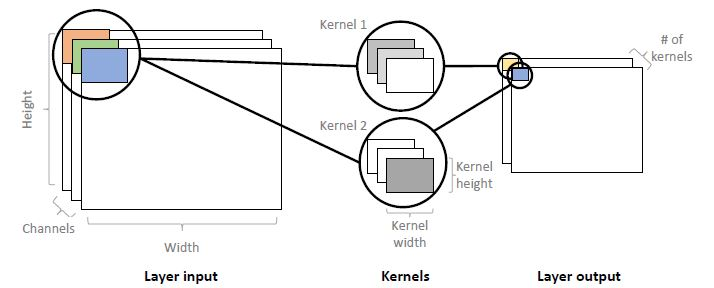
\includegraphics{figures/cnn.JPG}
  \caption{Convolution operation in CNN as shown in \cite{gal2016uncertainty}}
\end{figure*}

Recall the CNN structure mentioned in Fig 4.
The input to the i'th convolution layer is
expressed in more detail as a 3 dimensional tensor: 
\begin{equation*}
    x \in \mathbb{R}^{H_{i-1} \times W_{i-1} \times K_{i-1}}
\end{equation*}
with height $H_{i-1}$, width $W_{i-1}$, and $K_{i-1}$ channels. A convolution layer is then created by a sequence of $K_i$ kernels (weight tensors): $k_k \in R^{h \times w \times K_{i-1}}$
for k = 1, ...,$K_i$. Here we assume kernel height h, kernel width w, and the last dimension to match the number of channels in the input layer: $K_{i-1}$. Convolving the kernels with the input (with a given stride s) then results in an output layer of dimensions: 
\begin{equation*}
    y \in \mathbb{R}^{H'_{i-1} \times W'_{i-1} \times K_{i-1}} 
\end{equation*}
Each element $y_{i,j,k}$ is the sum of
the element-wise product of kernel $k_k$ with a corresponding patch in the input image x:
\begin{equation*}
    [[x_{i-h/2,j-w/2,1}, ..., x_{i+h/2,j+w/2,1}], 
\end{equation*}
\begin{equation*}
    ..., [x_{i-h/2,j-w/2,K_{i-1}} , ..., x_{i+h/2,j+w/2,K_{i-1}} ]]
\end{equation*}
Convolution is reformulated as a linear operation to integrate over the kernels. Let
$k_k \in \mathbb{R}^{h \times w \times K_{i-1}}$ for $k = 1, ...,K_i$ be the CNN’s kernels with height h, width w, and $K_{i-1}$
channels in the $i$’th layer. The input to the layer is represented as a 3 dimensional tensor
$x \in \mathbb{R}^{H_{i-1} \times W_{i-1} \times K_{i-1}}$ with height $H_{i-1}$, width $W_{i-1}$, and $K_{i-1}$ channels. It is analogous to extracting patches from the input and running a matrix product to merge the kernels with the input with
a given stride s: we extract and vectorize $h \times w \times K_{i-1}$ dimensional patches from the input with stride s.  Collecting the vectors in the matrix rows gives us a new representation of n patches for our input $\Bar{x} \in \mathbb{R}^{n \times hwK_{i-1}}$. 
The columns of the weight matrix $W i \in
\mathbb{R}^{hwK {i-1} \times K i}$ form the vectorized kernels.
The convolution operation is then the same as $\Bar{x}W I
\in \mathbb{R}^{n \times K i}$ of the matrix product.
The output columns can be rearranged to $y \in \mathbb{R}^{H i \times W_i
\times K_i}$ (since $n = H_i \times W_i$) in a 3-dimensional tensor.
On the $y$ matrix, pooling can
then be seen as a non-linear operation.
Notice that the operation of pooling is a non-linearity applied
to ReLU or Tanh non-linearities after the linear convolution equivalent\cite{kendall2019geometry}. 

We put a prior distribution over each kernel to turn the CNN into
a probabilistic model and roughly combine each kernel-patch pair with Bernoulli variational distributions.
The Bernoulli random variables $\epsilon_{i,j,n}$ are sampled and the weight matrix
$W_i$ · $diag([\epsilon_{i,j,n}]]^{{K_i}^{j=1}})$ is multiplied by patch n.
This product is analogous to an approximate distribution model with a different random variable
modelling each kernel-patch pair, tying the means of the random variables over the patches.
For multiple patches, the distribution
randomly sets kernels to 0.
This approximate distribution is also analogous to adding the
dropout before pool for each variable in the y tensor. 

\subsection{Bayes by Backprop}

The learning method of a
distribution of probability using the Neural network weights (Fig 5) play a major role in making results with better forecasts \cite{lee2020gradients}. Blundell et al. also suggested a novel and efficient algorithm called Bayes by Backprop (BBB) in order to calculate the volatility of these weights. \cite{blundell2015weight}

\begin{figure}[ht]
  \centering
  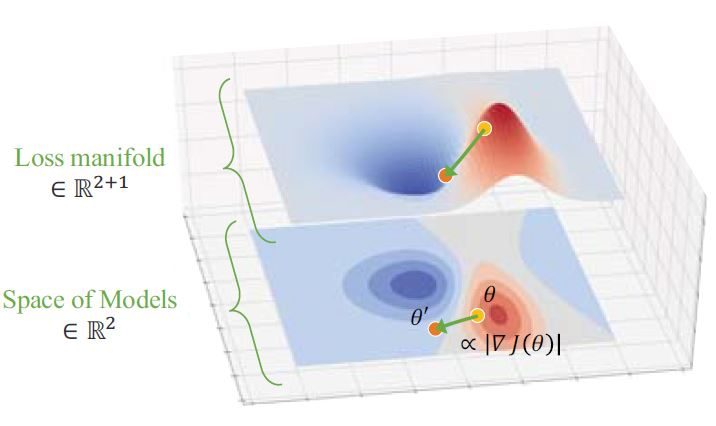
\includegraphics[scale=0.55]{figures/gd.JPG}
  \caption{Using stochastic gradient descent in back propogation.\cite{lee2020gradients}}
\end{figure}

The proposed BBB minimises the cost of compression known as variational
free energy (VFE) or the marginal probability of the lower bound.
They defined a cost function
to do so as follows: 

\begin{equation*}
    F(D,\theta) = KL[q(w|\theta)||P(w)] - \mathbb{E}_{q(w|\theta)}[logP(D|w)]
\end{equation*}

Ebrahimi et al. suggested a continuous uncertainty-guided approach to BNNs (named
UCB which stands for Uncertainty-guided continual learning technique with BNNs).
Continuous learning refers to learning a number of
new skills while impounding the gained information accumulated previously.
In order to formulate the shift in "important" parameters, both in setting a hard-threshold and
in a soft way, the proposed UCB exploits the expected uncertainty of the posterior distribution.
Recognition of multiple video behaviour involves not only
large data but is also a time-consuming process. \cite{kabir2018neural}

\begin{equation*}
    \theta = (\mu,\alpha),
\end{equation*}
\begin{equation*}
    \sigma^2 = \alpha.\mu^2,
\end{equation*}
\begin{equation*}
    q_\theta(w_{ijhwt}|D) = \mathcal{N}(\mu_{ijhwt},\alpha_{ijhwt}\mu^2_{ihjwt})
\end{equation*}

where $i$ represents the input, $j$ is the output, $h$ is the height of the
filter, $w$ is the width of the filter, and $t$ is the time dimension.
Ng et al. compared the performance of two well-known methods of uncertainty (MC dropout
and BBB) in medical image segmentation (cardiac MRI) on a UNet model in another study.
The results obtained showed that in the medical image
segmentation task, MC dropout and BBB showed almost similar performance. 


\section{Ensemble Techniques}
\subsection{Deep Ensemble}
Deep ensemble, another effective approach used to calculate uncertainty, has been used widely in many applications in the real world.
The data distributions in research datasets should be as
similar as the training datasets to achieve good learning outcomes.
The distributions of test datasets are unknown in many cases,
particularly in the case of an issue of uncertainty prediction \cite{pearce2018uncertainty}.
Therefore, it is impossible for conventional
learning methods to achieve competitive outcomes.
In order to figure out the uncertainty estimation issues, some researchers
applied MCMC and BNNs that focused on the prior distribution of datasets.
It becomes computationally expensive as these
techniques are used in large-scale networks. Using an ensemble of models(Fig 6) is a powerful approach which can be used to increase the predictive performance of supervised learners.
In order to get better predictions on test data, deep ensembles are implemented and model uncertainty estimates are also produced when OoD data is supplied with learning.\cite{pearce2018uncertainty}
The performance of models depends on the variance-reduction produced by combining
predictions that are individually susceptible to many types of errors.
Therefore, when using a large ensemble of multiple base models, the increase in
predictions is known, and such ensembles often produce distributional estimates of model uncertainty. \cite{abdar2020review}

\begin{figure}[ht]
  \centering
  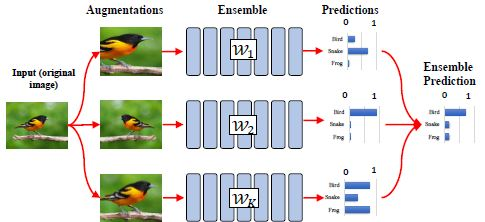
\includegraphics[scale=0.8]{figures/ensemble.JPG}
  \caption{Illustration of ensemble of models.\cite{abdar2020review}}
\end{figure}

A deep ensemble echo state network (D-EESN) model with two versions of the model for spatio-temporal forecasting and associated uncertainty measurement presented in \cite{pearce2018uncertainty}. The first framework applies a bootstrap ensemble approach and second one devised within a hierarchical Bayesian framework. Multiple levels of uncertainties and non-Gaussian data types were accommodated by general hierarchical Bayesian approach. The authors in broadened some of the deep ESN technique constituents
presented by Antonelo et al. and Ma et al. to fit in
a spatio-temporal ensemble approach in the D-EESN model
to contain such structure.

\subsection{Deep Ensemble Bayesian}

In literature, the expressive ability of
different ensemble techniques is widely demonstrated.
Traditional learning methods, however, have suffered from
many weaknesses and restrictions as described in[reference].
Fersini et al. used the ensemble learning technique to minimise the noise sensitivity associated with
language complexity to address these drawbacks, and it is possible to approximate more precise polarity estimation\cite{pearce2018uncertainty}.
Bayesian variable aggregation was used in the proposed ensemble process,
where both efficiency and instability of each single model is considered. 


One of the studies introduced one change to the prevalent approximate Bayesian inference by regularising parameters that could be set equal to the previous values obtained from a distribution \cite{gal2016uncertainty}. The method analysis indicated that the recovered posterior was appropriately oriented but leaned,to have underestimated marginal variance and overestimated correlation \cite{pearce2018uncertainty}.
One of the most interesting systems is Deep BAL (DBAL) with MC dropout to achieve uncertainty estimates \cite{abdar2020review}. In variational inference, Pop et al. argued that the mode collapse hypothesis was responsible for overconfident assumptions of DBAL methods in inference methods. They invented Deep Ensemble BAL that tackled the problem
of mode collapse and strengthened the process of MC dropout.


Pop et al. suggested a new AL technique in another review, especially for DNNs. To develop the state-of-the-art deep BAL technique that withstood the mode collapse problem, the statistical properties and expressive ability of model ensembles were used.\cite{pearce2018uncertainty}
Pearce et al., in another study, a new ensemble
of NNs, dubbed "anchored assembly," roughly Bayesian assembly approach.
The method suggested regularises the parameters of values collected from a distribution. 

\section{Applications in Robotics and Computer Vision}

Deep learning algorithms are still commonly used to map high-dimensional data to output arrays, though in many cases these mappings can be
incorrect, e.g. the incorrect labelling of two African Americans as gorillas in an image classification system has contributed to racial prejudice \cite{gal2016uncertainty}.
It is therefore important to take account of ambiguity, where
predictions are made by computer vision algorithms based on deep learning. 

To date, a range of research have discussed deep learning algorithm uncertainty for various uses, including but not limited to image/video retrieval, target detection,
semantic segmentation and scene comprehension, optical flow estimation and motion prediction, human pose estimation and re-identification and face recognition of pedestrian localization individuals, camera re-localization\cite{kwon2020uncertainty} some of which are shown in Fig 7).In fact, most research studies concentrate
on prediction accuracy in deep learning applications.Unlike certain studies, it has attracted significant interest to untangle the complexity
of different DNNs and address uncertainty for a variety of computer vision tasks\cite{kwon2020uncertainty}.
There is still a good record of using deep learning architectures in
Bayesian neural networks (BNNs) and Monte Carlo dropout (MC dropout) for uncertainty estimation.
MC dropout has been reported by nine studies as the
most efficient uncertainty quantity technique applicable to different deep learning architectures. 

\begin{figure*}
  \centering
  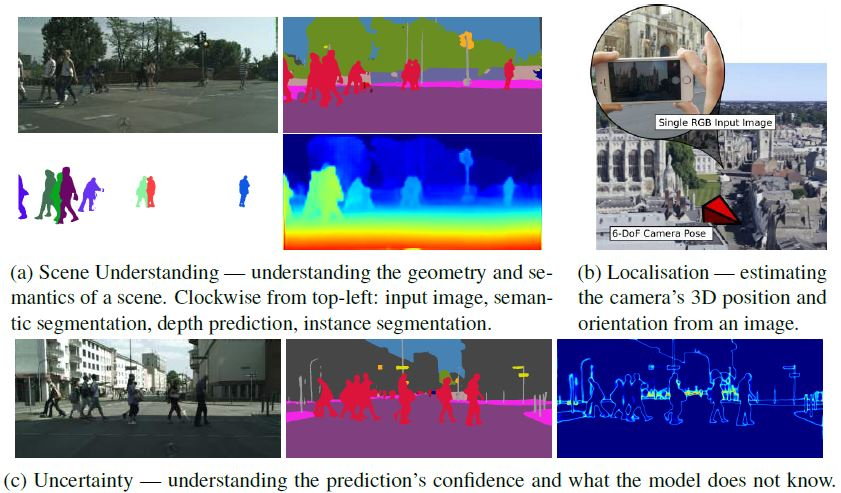
\includegraphics{figures/application.JPG}
  \caption{Computer Vision applications as shown in\cite{kendall2019geometry}.}
\end{figure*}

\subsection{Semantic Segmentation}

Three uncertainty quantification techniques were
examined by Bhandary et al., viz.
On the DarkNet21Seg 3D semantic segmentation model, MC-DropConnect, MC dropout and deep ensemble analysed the effect of various parameters
such as drop probability values on task performance, number of models in assemblies or forward passes and quality estimate uncertainty.
They showed that deep sets produced better results in
terms of uncertainty metrics and performance than other techniques\cite{dewan2017deep}. 

Kendall et al demonstrated that their Bayesian convolutionary neural networks model's uncertainty stemmed from the appearance
and present image dissimilarity to the training set and could estimate the re-localization uncertainty of the model\cite{kendall2017uncertainties}.

That enhanced the precision of
localization on a large outdoor dataset.
A measure of model uncertainty was developed by the same authors by MC sampling with
dropout and improved the performance of semantic segmentation compared to the state-of-the-art methods in 2016 \cite{loquercio2020general}. 

Weakly supervised semantic segmentation is achieved by
obtaining object response maps using image-level labels.
However, the predominant strategies rely on the classifier that can only engage in
discriminatory object regions in an answer map, as the network does not need seeing the entire object
for classification failure optimization\cite{petschnigg2021uncertainty}.
A principled and end-to-end training methodology was developed by Chang et al. to let the network
pay attention to other parts of the object, thus creating a more uniform and full response map.In the classification network, they explicitly suggested a mixup data augmentation technique and
formulated two terms of ambiguity regularisation to help function along with the mixup system \cite{petschnigg2021uncertainty}. 

\subsection{Autonomous Driving}
Kendall and Cipolla developed
working on autonomous vehicle applications
A picture taken from a front-facing camera mounted
in the vehicle offers tools for identifying a driver \cite{kendall2017uncertainties}.
This is a significant application as GPS systems
cannot always be trusted and offer low-accuracy localisation.
If used in autonomous driving, this positioning data can be used, for example\cite{petschnigg2021uncertainty},
to get details such as the distance of the vehicle from the sidewalk.
Following the tools built in the previous chapters, Kendall and Cipolla
measured model uncertainty and considered model uncertainty to correspond to positional error.  They found that test images from cars, pedestrians, or other objects with heavy occlusion resulted in high uncertainty,
with model uncertainty showing a linear pattern that increased with the distance from the training set (after calibration)\cite{petschnigg2021uncertainty}.
"Kendall et al. created models for scene understanding in further work, mapping objects on a pixel level in the pictures taken by the car to labels such as "pedestrian" or "cyclist".
Retrieving model uncertainty, they showed, for example,
that object edges have lower model confidence\cite{kendall2017uncertainties}.

\subsection{Image Segmentation}
In urban remote sensing images, Kampffmeyer et
al., for example, looked at semantic segmentation.
With the techniques mentioned, they used CNNs
and analysed the resulting complexity of segmentation \cite{loquercio2020general}.
Kampffmeyer et al. calculated the standard deviation
over 10 Monte Carlo samples' softmax outputs.
In order to achieve a single scalar value, they
then multiplied the standard deviation for all groups.
At object boundaries and in regions where the model is misclassified, they observed that model
uncertainty increased, validating the hypothesis that pixels with high model confidence are more often correctly identified. 
Kampffmeyer et al. also gave precision-recall plots showing that
classification accuracy improved as pixels with greater uncertainty were eliminated \cite{loquercio2020general}.
They concluded that uncertainty maps were a fair
estimate of the segmented remote sensing images' pixel-wise uncertainty. 


\section{Conclusion and Future Work}
Uncertainty analysis is an important step before deploying a machine learning model in any real-world application. This study has provided a thorough review of the most widely used uncertainty quantification methods. Nevertheless, it was also found that there is a lot of scope for future work. In spite of being out of the scope of this paper, it was found that the uncertainty analysis of machine learning models other that neural networks has not been done comprehensively. This might be due to the fact that neural networks are the state-of-the-art in many applications. Regarding approaches used for uncertainty quantification, information theory based methods were not included in this study which can be a solid future research direction. Moreover, uncertainty quantification of transfer learning and recently developed attention learning can also be part of the future research.

\bibliographystyle{IEEEtran}

\bibliography{agrosy} 


% that's all folks
\end{document}


